\documentclass[a0,11pt,portrait]{a0poster}

\usepackage[T1]{fontenc}                    % Ausgabekodierung
\usepackage[utf8]{inputenc}                 % Eingabekodierung
\usepackage[english]{babel}                 % Deutsch 

\usepackage{amsmath,amssymb,amsthm} % Math
\usepackage{stmaryrd}               % Lightning
\usepackage{multicol}

\setlength{\columnsep}{2cm}

\pagestyle{empty}
\setcounter{secnumdepth}{0}

\usepackage{xcolor}
\definecolor{oceangreen}{RGB}{0,75,90}

\usepackage{tikz}
\tikzstyle{vertex} = [circle, draw, fill=oceangreen!10,
  inner sep=2pt, minimum width=40pt]

\usepackage[absolute]{textpos}
\usepackage{graphicx}
\usepackage{fancybox}
\usepackage{wrapfig}
\usepackage{palatino}
\fontfamily{ppl}
\selectfont
\usepackage{url}

% see documentation for a0poster class for the size options here
\let\Textsize\normalsize
\def\Head#1{\noindent\hbox to \hsize{\hfil{\LARGE\color{oceangreen} #1}}\bigskip}
\def\LHead#1{\noindent{\LARGE\color{oceangreen} #1}\smallskip}
\def\Subhead#1{\noindent{\large\color{oceangreen} #1}}
\def\Title#1{\noindent{\VeryHuge\color{oceangreen!90} #1}}

\TPGrid[40mm,40mm]{15}{25}  % 3 - 1 - 7 - 1 - 3 Columns

\parindent=0pt
\parskip=0.5\baselineskip

\newcommand{\block}[1]{
\colorbox{oceangreen!10}{\parbox{\linewidth}{\vspace{0.5em}{\noindent #1}\vspace{0.25em}}}
}

% \textblockcolor{yellow}

\newcommand{\mycolwidth}{7.5}
\newcommand{\leftpos}{0}
\newcommand{\rightpos}{8}

\newcommand{\nul}{\textbf{0}}
\newcommand{\eins}{\textbf{1}}
\newcommand{\maxs}{\infty}
\newcommand{\id}{\text{id}}

\begin{document}

\begin{textblock}{12}(0,-0.25)
\resizebox{!}{1.5\TPVertModule}{
\includegraphics{ispunienfor.pdf}}
\end{textblock}

\begin{textblock}{2}(14,0.25)
\resizebox{!}{\TPVertModule}{
\includegraphics{logoispcmyk.pdf}}
\end{textblock}

\begin{textblock}{17}(-1,1.5)
\block{
\Huge
\color{oceangreen}
\hspace{1\TPHorizModule}Abstract Routing Models and Abstractions in the Context of Vehicle Routing}
\end{textblock}

\begin{textblock}{17}(-1,25.5)
\block{
\color{oceangreen}
\hspace{1\TPHorizModule}
Ren\'e Sch\"onfelder (\texttt{schoenfr@isp.uni-luebeck.de})
\hspace{3ex}and\hspace{3ex}Martin Leucker (\texttt{leucker@isp.uni-luebeck.de}),
\hfill July 6, 2012 \hspace{1\TPHorizModule}
}
\end{textblock}

\begin{textblock}{\mycolwidth}(\leftpos,2.5)
\LHead{Introduction} \\
\large
Various routing models each considering some aspects of finding ``best''
solutions:
\begin{itemize}
  \item Shortest Path Problem: Finding a shortest path also yields an efficient path regarding energy consumption.
  \item Shortest Weight-Constrained Path Problem: Optimize more than one target function, e.g.\ time and energy-consumption.
  \item Time-Dependent and Multi-Modal Routing: Finding shortest paths depending on the time, caused for example by including public transportation.
  \item Energy-Optimal Routing: Considering energy constraints for electric vehicles.
  \item Stochastic Routing: Minimizing expected costs, maybe given certain conditional probabilities.
  \item Rerouting: After finding an efficient path and turning to a different direction (or gaining additional information),
  quickly find an alternate efficient route.
\end{itemize}
Each model comes with its own set of algorithms,
our aim is to find a model unifying some aspects while still
allowing for most algorithms known for the shortest path problem.
\end{textblock}

\begin{textblock}{\mycolwidth}(\leftpos,8.25)
\LHead{Prototype} \\
The Technische Universit\"at M\"unchen (TUM) developed a prototypic routing service,
which is further developed at the University of L\"ubeck,
available at \url{www.isp.uni-luebeck.de/greennav}. It is used
to evaluate different routing algorithms. You can see a range prediction
of an electric vehicle.\\[1em]
\resizebox{5\TPHorizModule}{!}{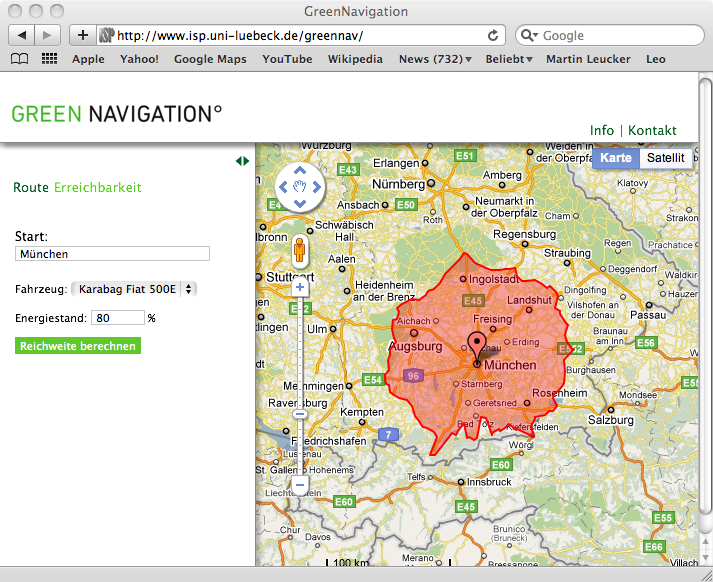
\includegraphics{greennav.png}}
\end{textblock}

\begin{textblock}{\mycolwidth}(\leftpos,14.75)
\LHead{Definition: State-Based Routing}
\begin{itemize}
  \item $G = (V, E)$ is a graph,
  \item $S$ is a set of states preordered by $\leq_S$,
  \item $\mathcal S:\ V \to \mathcal P(S)$ describes possible states at each vertex,
  \item $\mathbb W$ is a set of \emph{monotone} ($x_1 \leq_S x_2 \to f(x_1) \leq_S f(x_2)$)
  and \emph{extensive} ($x \leq_S f(x)$) weights $S \leadsto S$,
  \item $\mathcal W':\ E \to \mathbb W$ is a weighting,
\end{itemize}
such that
\begin{itemize}
  \item $\mathcal W'(x, y)$ is a weight $\mathcal S(x) \to \mathcal S(y)$, and
  \item the \emph{extension} of $\mathcal W'$ again is $\mathcal W:\ \text{walks} \to \mathbb W$ given by
  \[\mathcal W(\gamma) = \mathcal W'(v_0, v_1) \circ \ldots \circ \mathcal W'(v_{k-1}, v_k)\]
  for all walks $\gamma = (v_0, \ldots, v_k), k \geq 0$ (identity for $k = 0$).
\end{itemize}
\vspace{0.5em}
Objective:
\begin{itemize}
  \item Given $x, y \in V$ and initial state $s \in \mathcal S(x)$,
  find at least one corresponding path
  for each minimal element in $\min(\mathcal W(\text{walks from}\ x\ \text{to}\ y)(s))$
  (except for equivalence), where
  \[\min(S) := \{s \in S\ |\ \neg\exists s' \in S:\ s' < s\}.\]
\end{itemize}
\end{textblock}

\begin{textblock}{\mycolwidth}(\rightpos,2.5)
\LHead{The Theory} \\
There is a directed graph $G = (V, E)$ and a set of edge labels:
\begin{multicols}{2}
In a \emph{functional routing network} the edge labels are
functions on a semilattice $(S, \oplus, \leq)$, which can be
\begin{itemize}
  \item \emph{extensive}, if $\id_S \leq f$,
  \item \emph{right-inclining}, if $g \leq f \circ g$ for all $g \in F$,
  \item \emph{left-inclining}, if $f \leq f \circ g$ for all $g \in F$, and
  \item \emph{distributive}, if $f \circ (g \oplus h) = (f \circ g) \oplus (f \circ h)$
  for all $g, h \in F$.
\end{itemize}
In an \emph{algebraic routing network} the edge labels are elements from a semiring structure $(S, \oplus, \otimes, \leq, \nul, \eins)$, for example a \emph{bounded dioid}:
\begin{itemize}
  \item $(S, \oplus, \otimes, \nul, \eins)$ is a semiring
  \item $\leq$ is the partial order of the semilattice $(S, \oplus)$,
  \item $\oplus$ is idempotent, i.e.\ $a \oplus a = a$, and
  \item $\eins \oplus a = a \oplus \eins = \eins$.
\end{itemize}
\end{multicols}
Problem: Find a best paths between two vertices w.r.t.~the partial order $\leq$ of the semilattice given a starting value.

\emph{Profile search}: Find best paths for all starting values.

\textbf{Theorem about profile searches}:
The profile searches on functional routing networks with
\emph{extensive, inclining and distributive}
functions are algebraic routing problems on \emph{bounded dioids}.
\end{textblock}

\begin{textblock}{\mycolwidth}(\rightpos,9)
\LHead{Algebraic Abstractions} \\
\begin{center}
\begin{tikzpicture}[scale=4]
\node[] (x) at (0, 0) {$0.43$};
\node[] (a2) at (-3.5, 0) {$4$};
\node[] (a1) at (3.5, 0) {$1$};
\node[] (fx) at (0, -1.5) {$0.7 \leq 0.74 \leq 2$};
\node[] (fa2) at (-3.5, -1.5) {$7$};
\node[] (fa1) at (3.5, -1.5) {$2$};
\draw[->] (x) -- (a2) node[midway, above]
  {$\alpha^\downarrow(a) = \lfloor 10 a \rfloor$};
\draw[->] (x) -- (a1) node[midway, above]
  {$\alpha^\uparrow(a) = \lceil a \rceil$};
\draw[->] (x) -- (fx) node[midway, right] {$+ 0.31$};
\draw[->] (a1) -- (fa1) node[midway, left] {$+1$};
\draw[->] (a2) -- (fa2) node[midway, right] {$+3$};
\draw[->] (fa1) -- (fx) node[midway, below]
  {$\gamma^\uparrow(a) = a$};
\draw[->] (fa2) -- (fx) node[midway, below]
  {$\gamma^\downarrow(a) = \frac{a}{10}$};
\end{tikzpicture}
\end{center}
\end{textblock}

\begin{textblock}{\mycolwidth}(\rightpos,17.2)
\LHead{Conclusions and Future Work} \\
First tests yielded reasonable results, but we just started to implement
various shortest path algorithms for the state-based routing problem and
its profile version. Hence runtime and space analyzations are near future
goals. The model itself is promising, comprising time-dependent routing,
battery constraints, stochasticity and multi-criteria routing, but the
running time is an important question to answer soon.

In the long run we aim to extend GreenNav by more sophisticated algorithms
and services. An egoistic routing algorithm is but the first step towards
ecological sustainability. Multi-modality and stochasticity are two important
points to consider.
\end{textblock}

\begin{textblock}{15}(0,20.9)
\line(1,0){2160}
\end{textblock}

\begin{textblock}{15}(0,21)
\begin{multicols}{3}
\renewcommand{\refname}{\normalfont\LHead{Related Work}\vspace{-1cm}}
\nocite{*}
\bibliographystyle{plain} %plain
\bibliography{ref}
\end{multicols}
\end{textblock}

\end{document}